\chapter{Results}\label{ch4}

To understand the process better, we have evaluated the shape fitting and the color fitting module separately. The dataset we evaluate is exclusively based on captures made by the D415 camera, it includes images with varying faces, poses and illumination conditions. Around 80\% of the dataset consists of frontal shots, the rest of the images are varying between $\pm 30^{\circ}$ yaw and roll rotation angles. To replicate the real world scenarios as close as possible, we did not set up a specific camera rig for capturing procedure, rather, photos are taken arbitrarily. To compare our results to the previous results we have also executed a novel 2D fitting  \cite{Schoenborn2017} over the same dataset. Unfortunately, we were unable to run \cite{betschard2016} project and therefore the values that we list are directly taken from the report — those values are not tested on our dataset. Before we present our results, we shall define the evaluation metrics that we employ to assess the performance and quality of the final reconstructions. 

\section{Evaluation Metrics}
The most obvious and straightforward way to evaluate the shape quality of 3D object reconstruction is to measure the distance between the target object and the reconstructed one. Thanks to the target mesh we have obtained from the camera and the reconstructed mesh produced after the 3DMM fitting, we have a possibility to work with 3D mesh objects and evaluate the distance between them. The more robust and meaningful distance measure is the average mesh distance. It measures the distance from every point on one mesh to the closest point on another mesh and averages them. This kind of evaluation metrics are known to work well when two objects that are being evaluated are symmetric. Unfortunately, in our case, the target mesh and the reconstructed meshes are far from symmetric and quite a lot of outlier points are observed. Therefore, to make the returned value reasonable we have made a small adjustment. We employ the simple boundary point ignorance technique, which ignores the distance entry for every point on one mesh that has its closest point located on the boundary of another mesh. This will ignore obvious outliers and give us a quantitative measure of how far our shape reconstruction is from the real shape. The method is robust enough and works well even when the mesh points are distributed non-evenly. When it comes to image evaluation, the best way to evaluate it is using human perception. Therefore, we make sure to provide a set of sample reconstructions alongside numerical measurements.

\section{Shape Fitting Module Evaluation}
We first start listing results of shape fitting module and evaluating how well reconstructed shape fits to the target mesh. Table \ref{t4.1} shows the average mesh reconstruction accuracy in millimeters after 1000 shape fitting iterations. 

\begin{table}[h]
  \centering
  \begin{tabular}{ c|c|c }
      Evaluated Against & \#Iterations & Avg. Mesh Distance [mm]\\
      \hline
      Target Mesh & 1000  & \textbf{1.18} \\
      Ground Truth & 1000 & \textbf{1.47} \\
      \hline
  \end{tabular}
  \caption{Shape fitting accuracy in mm.}
  \label{t4.1}
\end{table}

The value for the ground truth alignment is obtained by aligning the best shape reconstruction over the ground truth using the method described previously, however, we do not perform any explicit alignment procedure for the shape fit and the target mesh because the shape fitting itself is an alignment problem. The latter also explains the difference between those two evaluations - shape fit is constantly getting evaluated against the target mesh so it is expected that the average value would be lower between the target mesh and the reconstructed mesh than the average value between the ground truth and the reconstructed mesh. 

\begin{figure}[h]
  \centering
  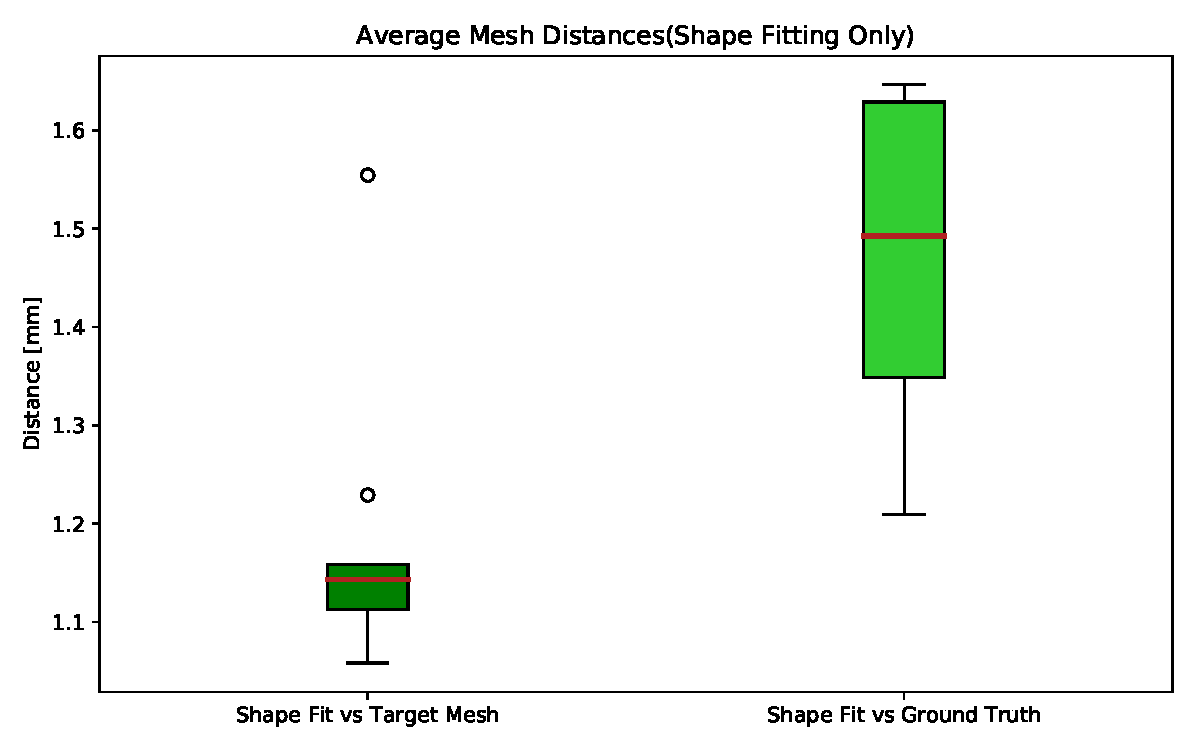
\includegraphics[width=\textwidth]{Figures/shapeFittingPlot.pdf}
  \caption{The first column of this box plot shows the average mesh distance between the best shape fit and the target mesh, the second column shows the distance between the best shape fit and the ground truth. The red line indicates the median (Table \ref{t4.1}).}
  \label{f4.1}
\end{figure}

Figure \ref{f4.1} shows the distribution of the entire dataset.  Outlier points in the first column are produced by $\pm 30^\circ$ yaw rotated shots. As we have emphasized previously our method performs noticeably better in the frontal shots and the worst in shots where the yaw rotation is introduced. The reason behind this goes back to the landmark detection procedure. Recall, we detect landmarks onto a color image and then de-project landmark pixels to points. The problem occurs due to the fact that whenever the Dlib landmark detection library detects a face, it provides the full set of landmarks without respecting the pose. If the part of the face is not visible, landmarks that are located onto the occluded side of the face are still present. Those landmarks are first not very accurate and secondly, they are getting grouped into one area and the distance between landmark points does not correspond to the actual distance.  This either breaks our shape fitting part or produces bad reconstructions, because of this constraint majority of our dataset samples are frontal shots. In Figure \ref{f4.2} we show two sample shape reconstruction after 1000 iterations. 

\begin{figure}
  \centering
  \begin{minipage}{.325\textwidth}
    \centering
    \caption*{X Slice}
    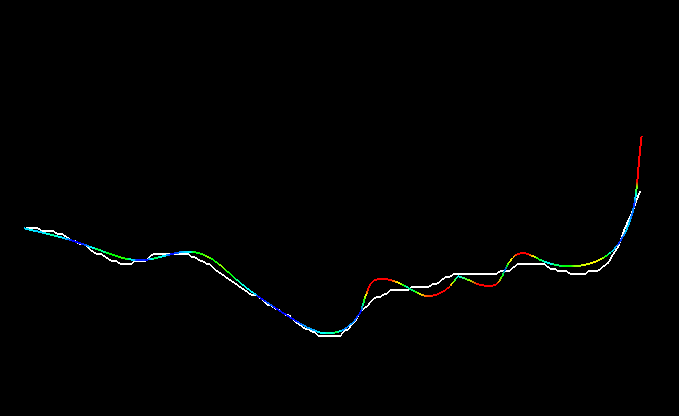
\includegraphics[width=0.99\textwidth]{Figures/eval/our/3/x.png}
  \end{minipage}
  \begin{minipage}{.325\textwidth}
    \centering
    \caption*{Y Slice}
    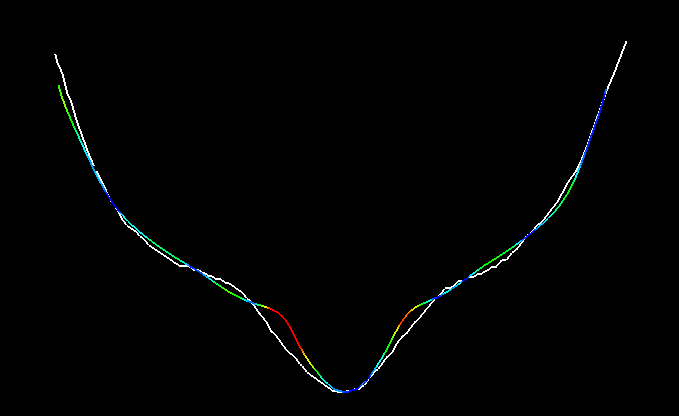
\includegraphics[width=0.99\textwidth]{Figures/eval/our/3/y.png}
  \end{minipage}
  \begin{minipage}{.325\textwidth}
    \centering
    \caption*{Z Slice}
    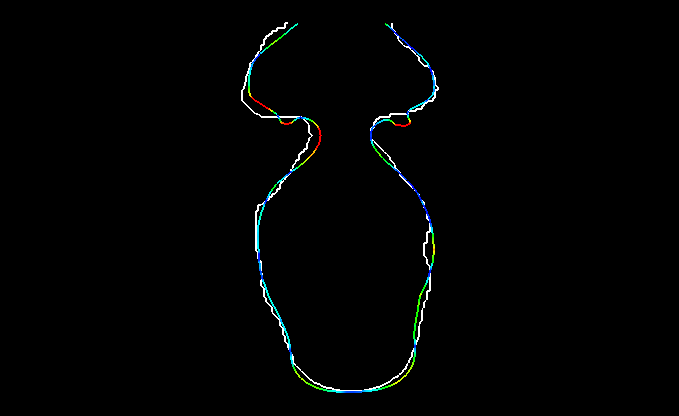
\includegraphics[width=0.99\textwidth]{Figures/eval/our/3/z.png}
  \end{minipage}

  \begin{minipage}{.325\textwidth}
    \centering
    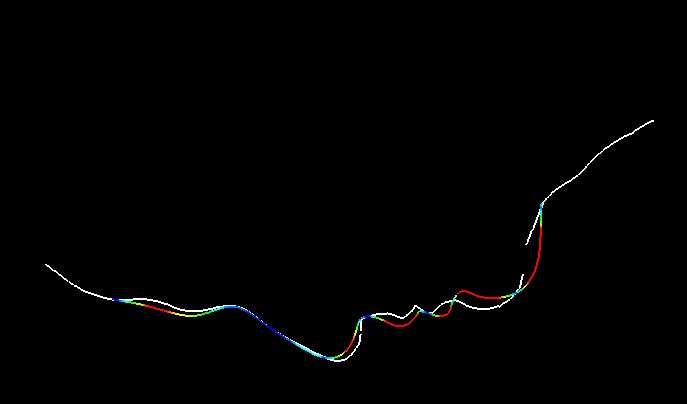
\includegraphics[width=0.99\textwidth]{Figures/eval/our/3/x-gt.png}
  \end{minipage}
  \begin{minipage}{.325\textwidth}
    \centering
    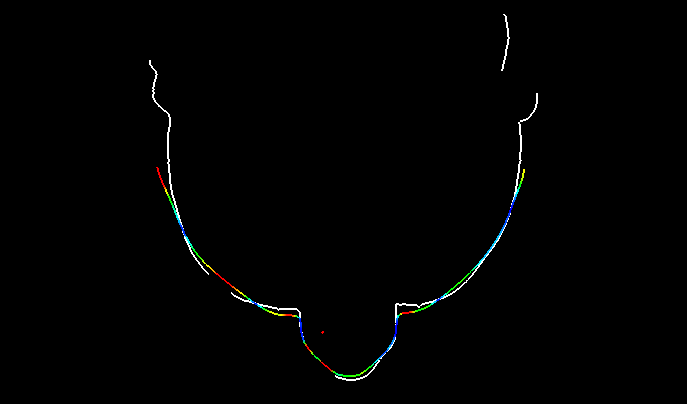
\includegraphics[width=0.99\textwidth]{Figures/eval/our/3/y-gt.png}
  \end{minipage}
  \begin{minipage}{.325\textwidth}
    \centering
    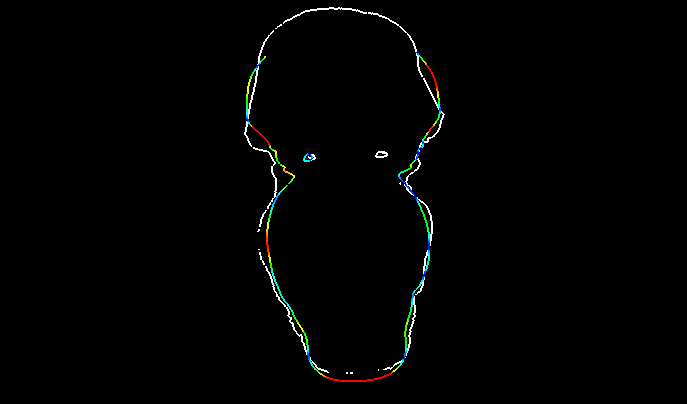
\includegraphics[width=0.99\textwidth]{Figures/eval/our/3/z-gt.png}
  \end{minipage}

  Sample 1

  \begin{minipage}{.325\textwidth}
    \centering
    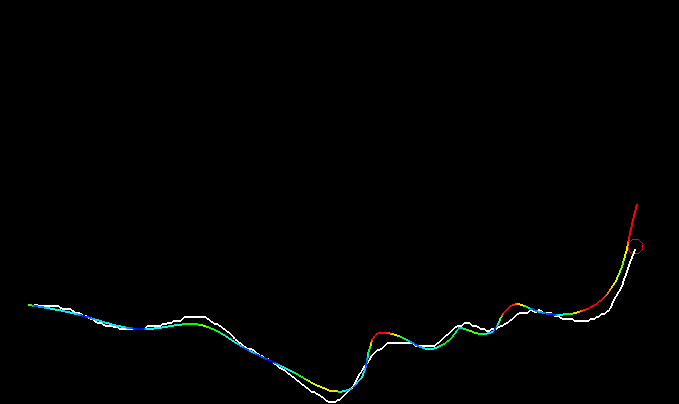
\includegraphics[width=0.99\textwidth]{Figures/eval/our/1/x.png}
  \end{minipage}
  \begin{minipage}{.325\textwidth}
    \centering
    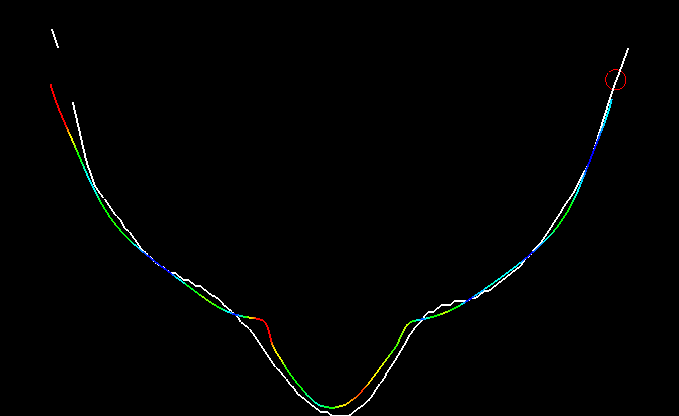
\includegraphics[width=0.99\textwidth]{Figures/eval/our/1/y.png}
  \end{minipage}
  \begin{minipage}{.325\textwidth}
    \centering
    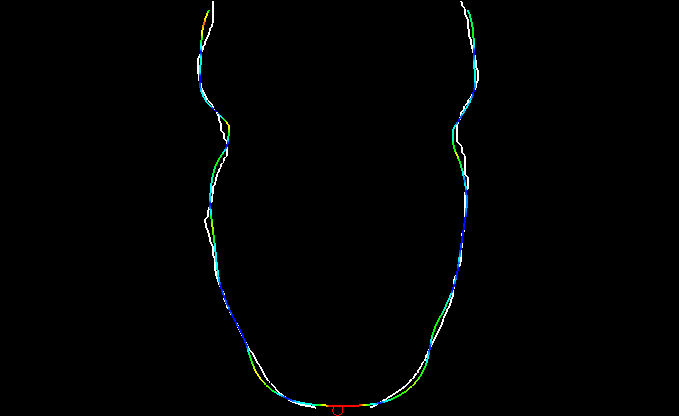
\includegraphics[width=0.99\textwidth]{Figures/eval/our/1/z.png}
  \end{minipage}

  \begin{minipage}{.325\textwidth}
    \centering
    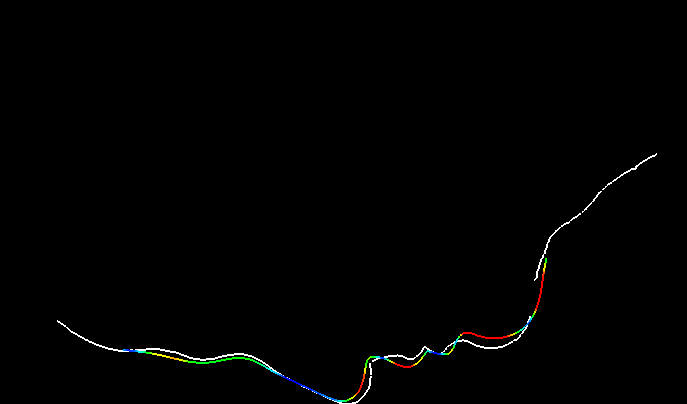
\includegraphics[width=0.99\textwidth]{Figures/eval/our/1/x-gt.png}
  \end{minipage}
  \begin{minipage}{.325\textwidth}
    \centering
    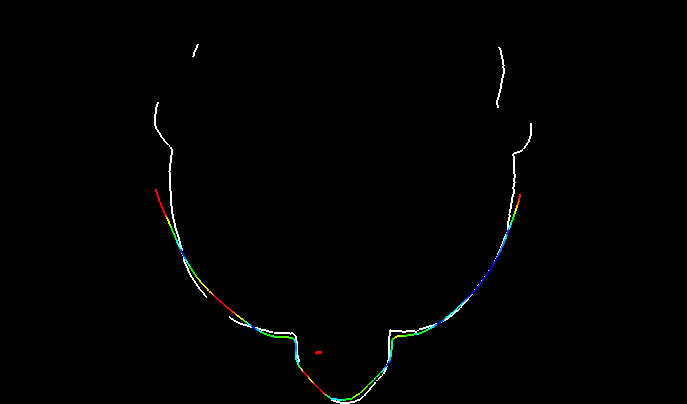
\includegraphics[width=0.99\textwidth]{Figures/eval/our/1/y-gt.png}
  \end{minipage}
  \begin{minipage}{.325\textwidth}
    \centering
    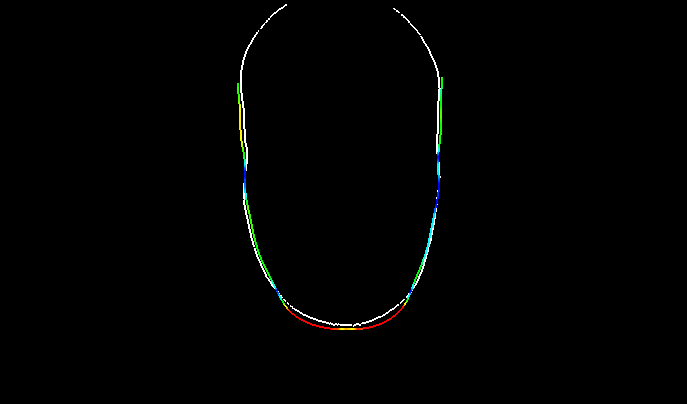
\includegraphics[width=0.99\textwidth]{Figures/eval/our/1/z-gt.png}
  \end{minipage}

  Sample 2

  % \begin{minipage}{.325\textwidth}
  %   \centering
  %   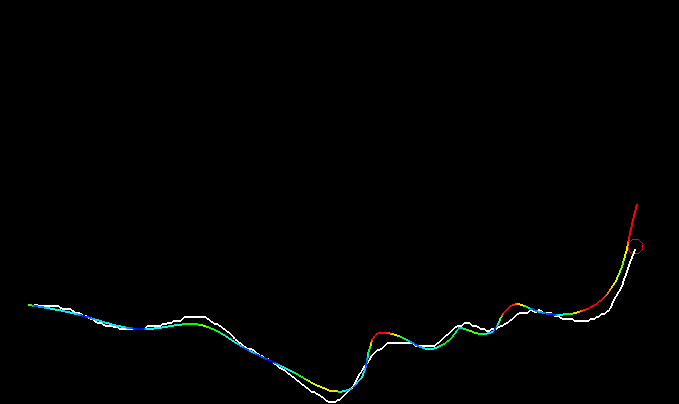
\includegraphics[width=0.99\textwidth]{Figures/eval/our/1/x.png}
  % \end{minipage}
  % \begin{minipage}{.325\textwidth}
  %   \centering
  %   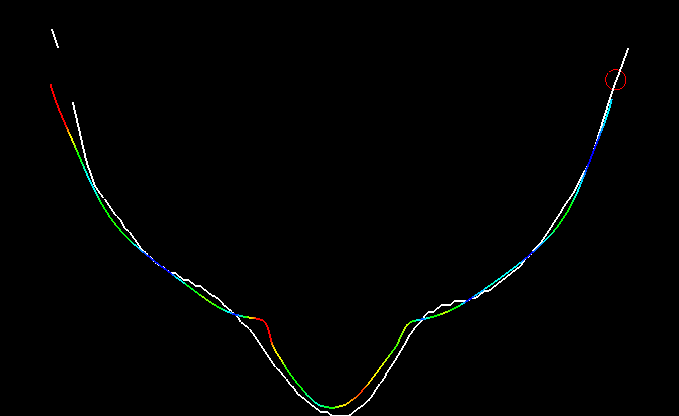
\includegraphics[width=0.99\textwidth]{Figures/eval/our/1/y.png}
  % \end{minipage}
  % \begin{minipage}{.325\textwidth}
  %   \centering
  %   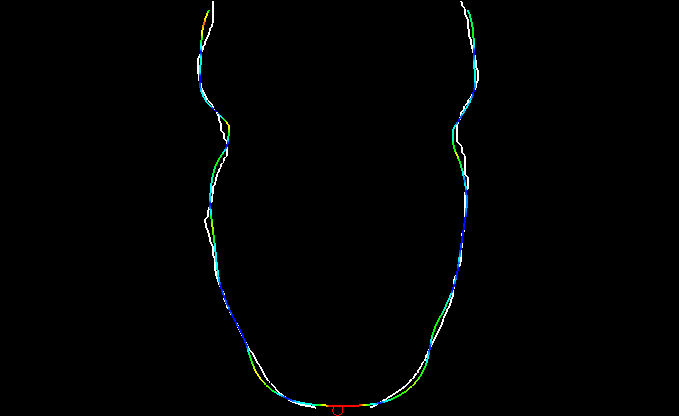
\includegraphics[width=0.99\textwidth]{Figures/eval/our/1/z.png}
  % \end{minipage}

  % \begin{minipage}{.325\textwidth}
  %   \centering
  %   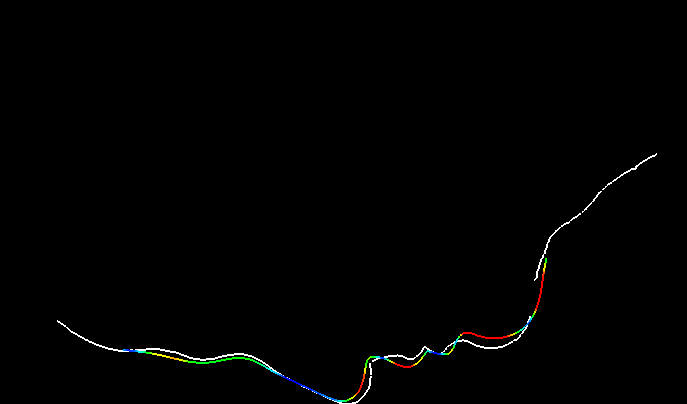
\includegraphics[width=0.99\textwidth]{Figures/eval/our/1/x-gt.png}
  % \end{minipage}
  % \begin{minipage}{.325\textwidth}
  %   \centering
  %   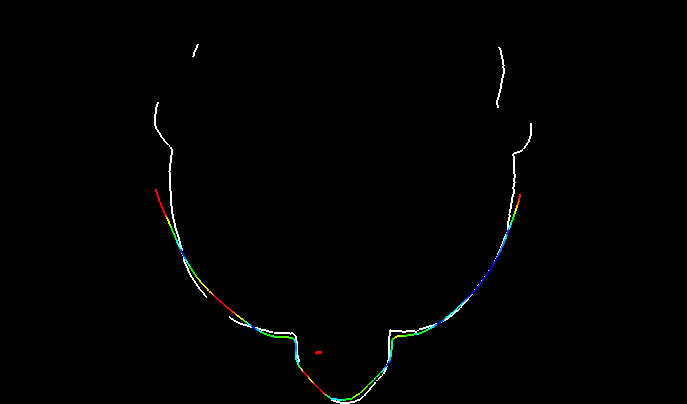
\includegraphics[width=0.99\textwidth]{Figures/eval/our/1/y-gt.png}
  % \end{minipage}
  % \begin{minipage}{.325\textwidth}
  %   \centering
  %   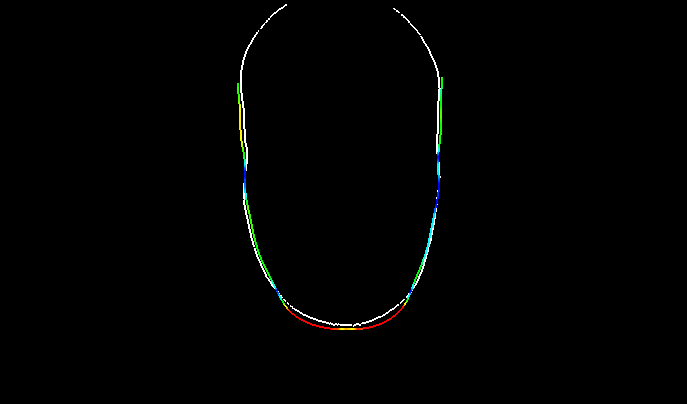
\includegraphics[width=0.99\textwidth]{Figures/eval/our/1/z-gt.png}
  % \end{minipage}
  % Sample 3
  \caption{The first row of these two sample fits shows the target and the best shape fit alignment, the second ground truth and the best shape fit. In both cases, the colored line represents the best shape fit instance, where the blue color indicates 0.0 mm distance between the points and the red indicates 3.0 mm+ distance. Both shots are frontal shots to make the slice visualization easier to understand.}
  \label{f4.2}
\end{figure}

As we can clearly see from the sample slices above, the highest errors (colored in red) are being accumulated in places where there are a lot of curvature or acute angles. For example the lip details or nose angle. This is because the point cloud itself does not capture this kind of details, what we have instead is a rather smooth and generic shape without detailed facial features.  

\section{Full Fitting Evaluation (Shape Fitting + Color Fitting)}
Once the shape fitting module ends its cycle the final reconstruction and other necessary parameters are then being passed to the color fitting module. It starts another proposal-and-verify cycle to approximate the color values from the target image. Figure \ref{f4.3} shows the comparison of the shape reconstruction quality after the shape fitting and after the full fitting.

\begin{figure}
  \centering
  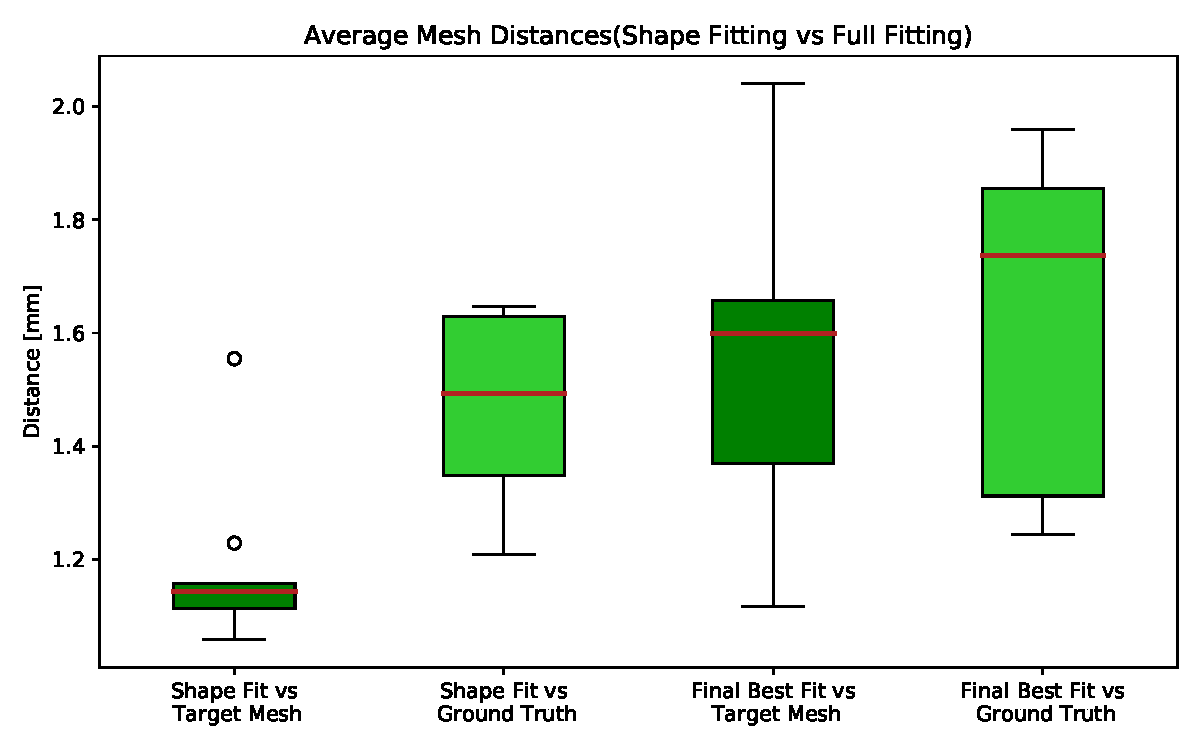
\includegraphics[width=\textwidth]{Figures/our.pdf}
  \caption{The average mesh distances after the shape fitting only (1st and 2nd column) and after the full fitting (3rd and 4th column). The first and third column shows the average mesh distances between the reconstructed mesh and the target mesh, the second and fourth column shows the average mesh distances between the reconstructed mesh and the ground truth.}
  \label{f4.3}
\end{figure}

As stated previously, if we do not add shape or pose proposals to the color fitting module, obviously the average distance will not change. While numerically this would be perfect, visually we would not get satisfactory results. Because of this, we had to make a compromise and include shape and pose parameter proposals into the color fitting module. Even though we evaluate landmark positions and mirror the point cloud evaluator from the shape fitting module, shape still gets worst in comparison to the shape fitting results.\bigskip

Alongside our fitting module, we have evaluated a novel 2D fitting approach\footnote{Basel Face Registration Pipeline — \url{https://github.com/unibas-gravis/basel-face-pipeline/}}. To do so, we took our entire dataset images and obtained landmarks for each target image using the \textit{landmarks-clicker}\footnote{Landmarks Clicker
— \url{https://github.com/unibas-gravis/landmarks-clicker/}} tool. We did not make any changes to the standard fitting module, we simply pass our dataset images with corresponding landmarks to the script, and in the end, evaluate the final reconstructions. Table \ref{t4.2} shows the result of the final average shape reconstruction accuracy calculated against the ground truth.\bigskip

\begin{table}[h]
  \centering
  \begin{tabular}{ c|c|c }
      Landmarks  & Shape Information & Avg. Mesh Distance [mm]\\
      \hline
      2D   & No  & 2.21 \cite{Schoenborn2017}\\
      3D   & Yes(Depth) & 1.94 \cite{betschard2016}*\\
      3D   & \textbf{Yes(Point Cloud)} & \textbf{1.61} \\
      \hline
  \end{tabular}
  \caption{The final shape fitting accuracy in mm obtained by aligning the final 3D reconstructions over the ground truth. *BFM dataset evaluation value; taken directly from the paper to have a rough idea how does our method compare to it — we did not manage to run the module to test it on our dataset.}
  \label{t4.2}
\end{table}

Table \ref{t4.3} shows the average distance between the final shape fit and the target mesh. This value is obtained by aligning the final reconstruction and the corresponding target mesh. \bigskip

\begin{table}[h]
  \centering
  \begin{tabular}{ c|c|c }
      Landmarks  & Shape Information & Avg. Mesh Distance [mm]\\
      \hline
      2D   & No  & 2.94 \cite{Schoenborn2017}\\
      3D   & \textbf{Yes(Point Cloud)} & \textbf{1.56} \\
      \hline
  \end{tabular}
  \caption{Final shape fitting accuracy in mm obtained by aligning the final 3D reconstructions over the target mesh.}
  \label{t4.3}
\end{table}

Figure \ref{f4.5} shows the visual comparison of the target image, rendered model fit of our method and standard fitting method. Figure \ref{f4.6} shows the same results as Figure \ref{f4.5} but the final fit is overlaid to the target image to make the comparison easier. We argue that the reconstructions that are produced by our method are capturing a bit more details and facial characteristics, whereas the standard fitting results are more generic while still maintaining close-to-target state. We think that this is because our shape reconstruction quality is noticeably better and hence after applying the texture and illumination we get a bit more close to the target results. We once again emphasize and more closely observe(rows 3 and 4) the difficulties our method experiences when working with poses that have yaw rotation applied.\bigskip

The box plot in Figure \ref{f4.4} shows the distribution of the average mesh distances of the entire dataset. Where the first and second columns indicate our final shape reconstruction accuracies, and the third and fourth column indicate the performance of the standard fitting method. Unlike results that we have listed for the shape fitting evaluation, this time, the final fits are being aligned both to the target mesh and the ground truth mesh. 

\begin{figure}[h]
    \centering
    \begin{minipage}{.325\textwidth}
      \centering
      \caption*{Target Image}
      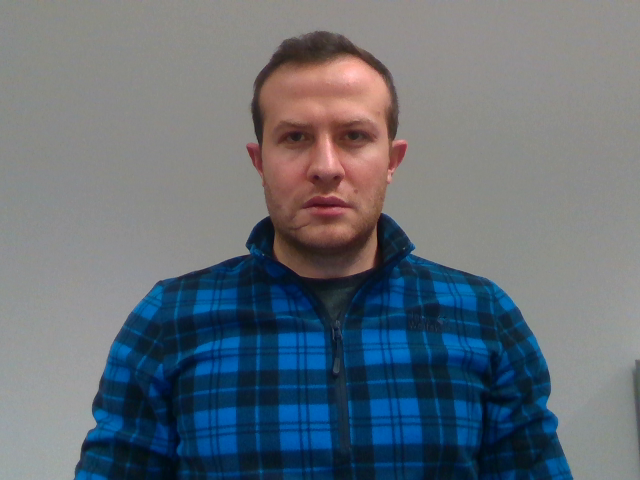
\includegraphics[width=0.99\textwidth]{Figures/dataset/target/1.png}
    \end{minipage}
    \begin{minipage}{.325\textwidth}
      \centering
      \caption*{\textbf{Our Fit}}
      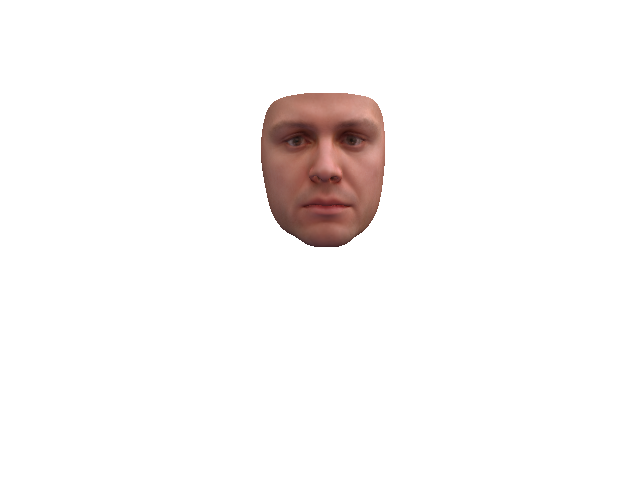
\includegraphics[width=0.99\textwidth]{Figures/dataset/our/1.png}
    \end{minipage}
    \begin{minipage}{.325\textwidth}
      \centering
      \caption*{Standard Fit}
      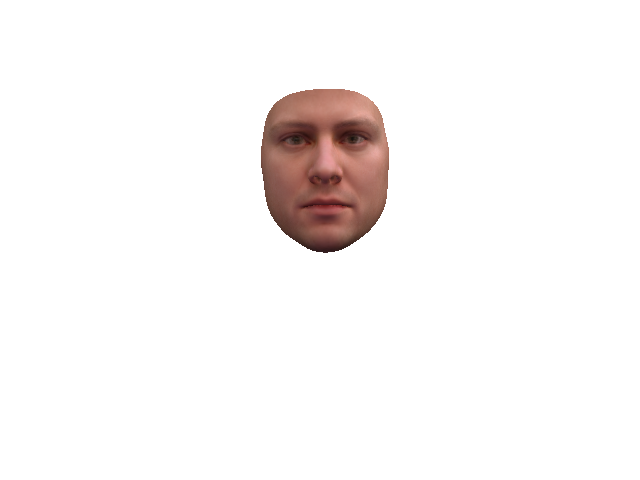
\includegraphics[width=0.99\textwidth]{Figures/dataset/2D/1.png}
    \end{minipage}

    \begin{minipage}{.325\textwidth}
      \centering
      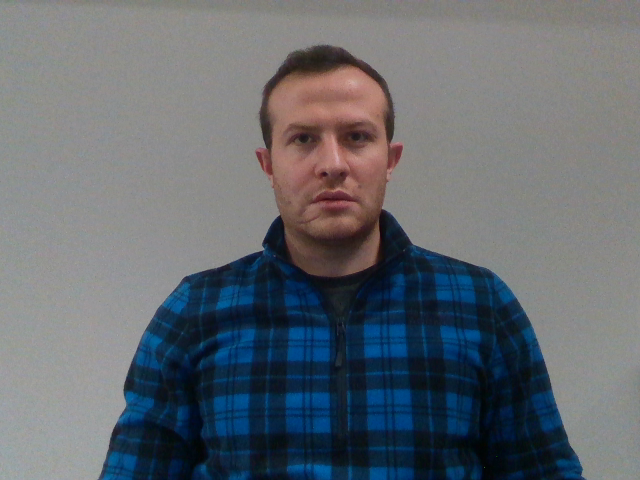
\includegraphics[width=0.99\textwidth]{Figures/dataset/target/3.png}
    \end{minipage}
    \begin{minipage}{.325\textwidth}
      \centering
      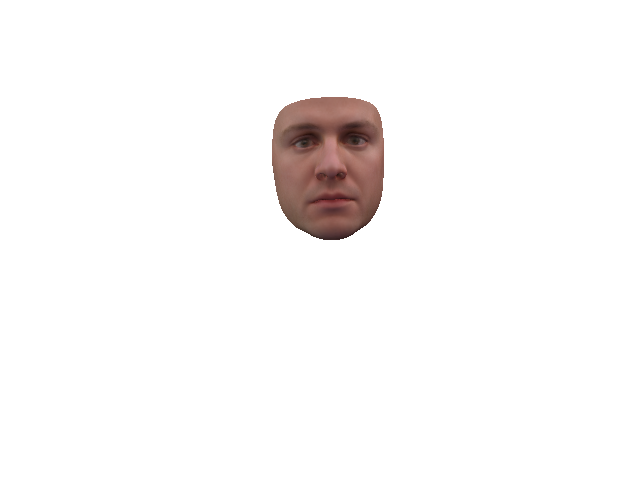
\includegraphics[width=0.99\textwidth]{Figures/dataset/our/3.png}
    \end{minipage}
    \begin{minipage}{.325\textwidth}
      \centering
      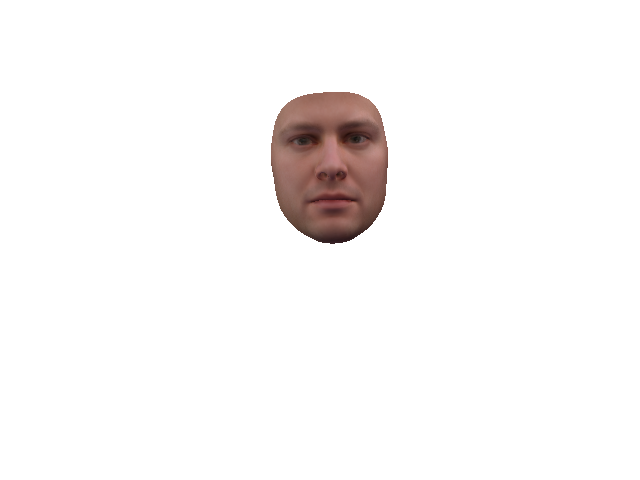
\includegraphics[width=0.99\textwidth]{Figures/dataset/2D/3.png}
    \end{minipage}

    \begin{minipage}{.325\textwidth}
      \centering
      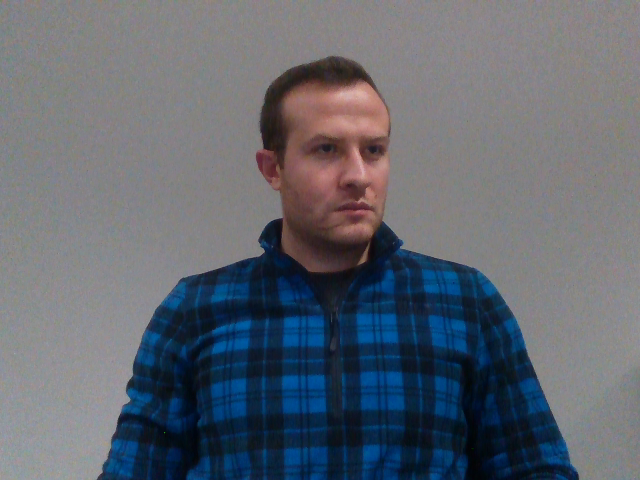
\includegraphics[width=0.99\textwidth]{Figures/dataset/target/4.png}
    \end{minipage}
    \begin{minipage}{.325\textwidth}
      \centering
      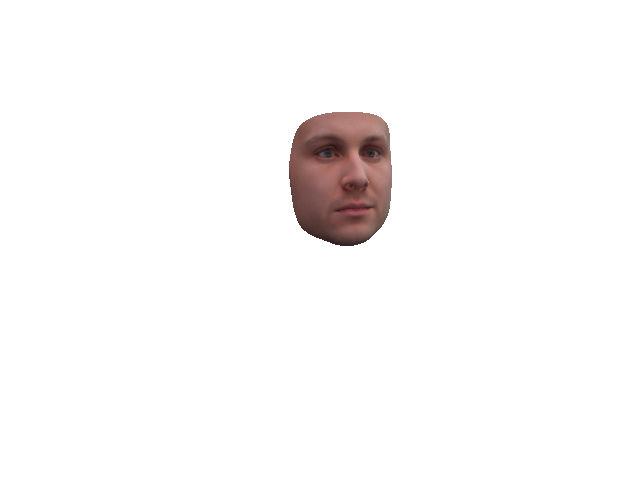
\includegraphics[width=0.99\textwidth]{Figures/dataset/our/4.png}
    \end{minipage}
    \begin{minipage}{.325\textwidth}
      \centering
      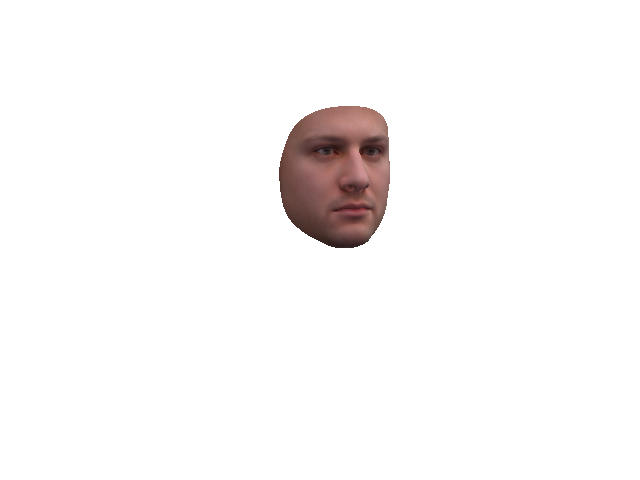
\includegraphics[width=0.99\textwidth]{Figures/dataset/2D/4.png}
    \end{minipage}

    \begin{minipage}{.325\textwidth}
      \centering
      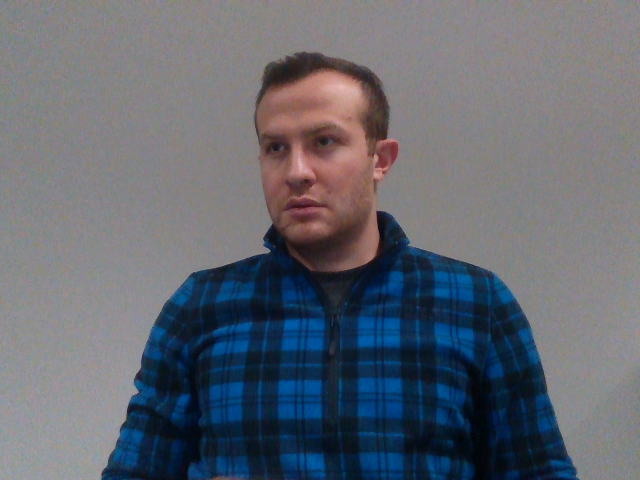
\includegraphics[width=0.99\textwidth]{Figures/dataset/target/5.png}
    \end{minipage}
    \begin{minipage}{.325\textwidth}
      \centering
      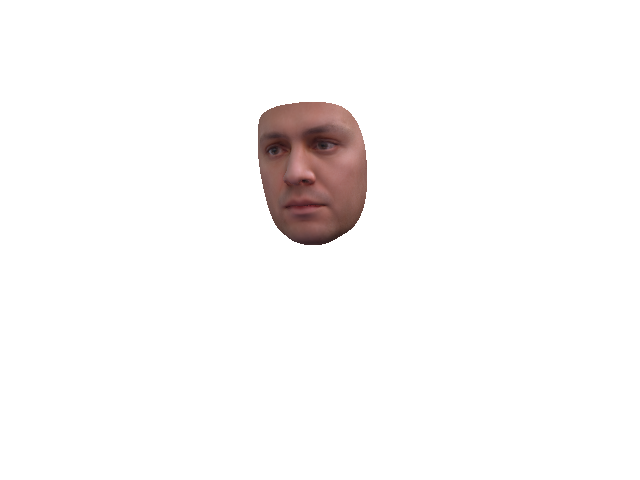
\includegraphics[width=0.99\textwidth]{Figures/dataset/our/5old.png}
    \end{minipage}
    \begin{minipage}{.325\textwidth}
      \centering
      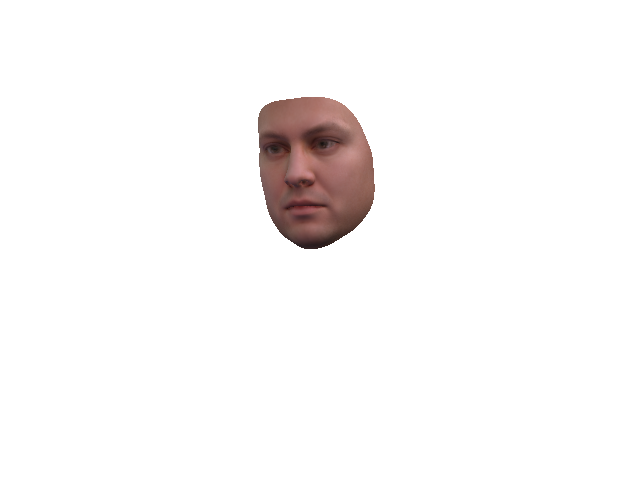
\includegraphics[width=0.99\textwidth]{Figures/dataset/2D/5.png}
    \end{minipage}

    \begin{minipage}{.325\textwidth}
      \centering
      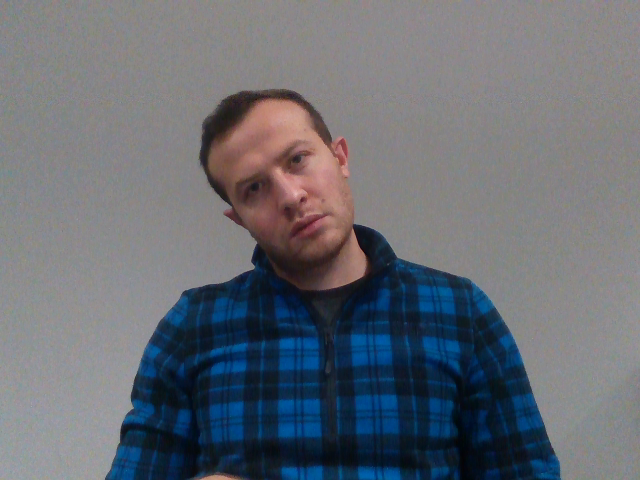
\includegraphics[width=0.99\textwidth]{Figures/dataset/target/6.png}
    \end{minipage}
    \begin{minipage}{.325\textwidth}
      \centering
      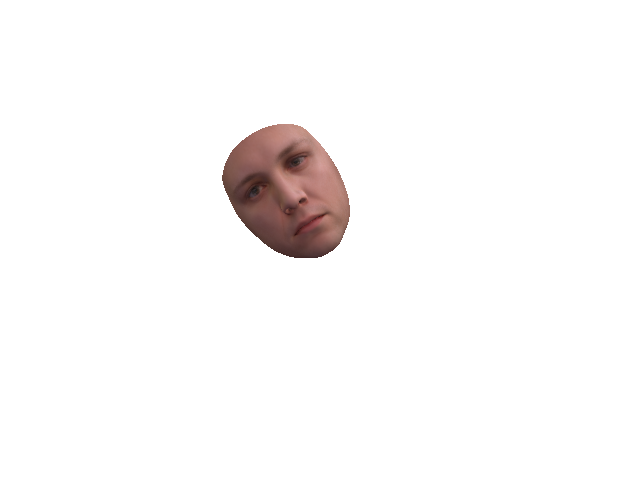
\includegraphics[width=0.99\textwidth]{Figures/dataset/our/6.png}
    \end{minipage}
    \begin{minipage}{.325\textwidth}
      \centering
      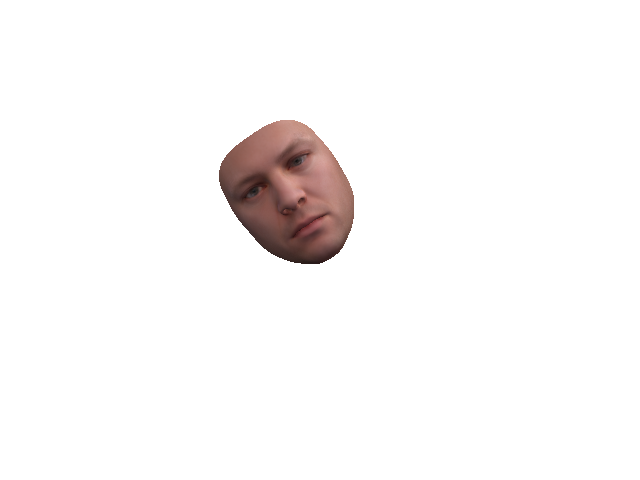
\includegraphics[width=0.99\textwidth]{Figures/dataset/2D/6.png}
    \end{minipage}

    \begin{minipage}{.325\textwidth}
      \centering
      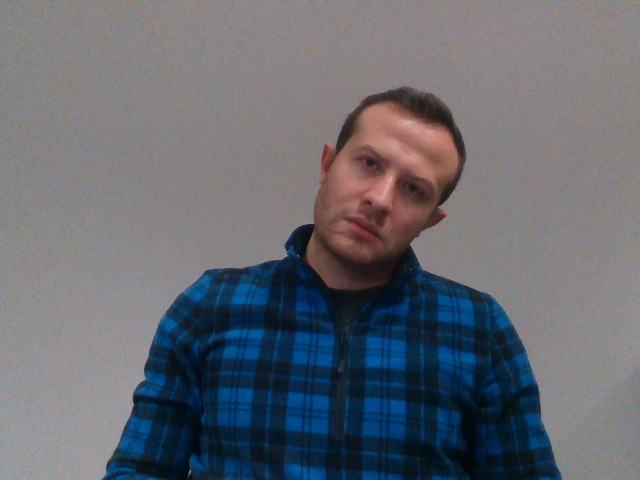
\includegraphics[width=0.99\textwidth]{Figures/dataset/target/7.png}
    \end{minipage}
    \begin{minipage}{.325\textwidth}
      \centering
      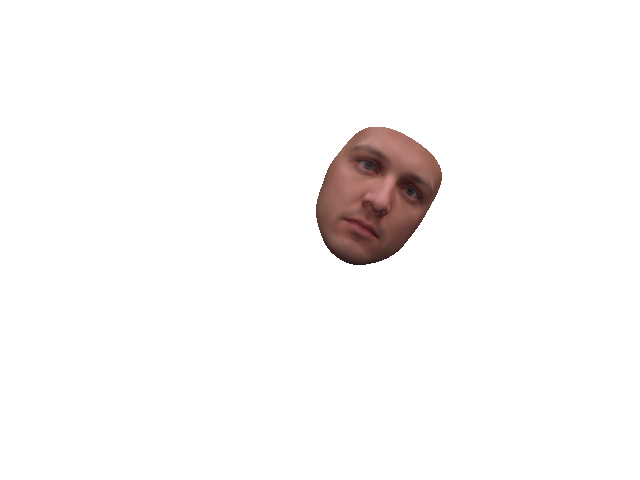
\includegraphics[width=0.99\textwidth]{Figures/dataset/our/7.png}
    \end{minipage}
    \begin{minipage}{.325\textwidth}
      \centering
      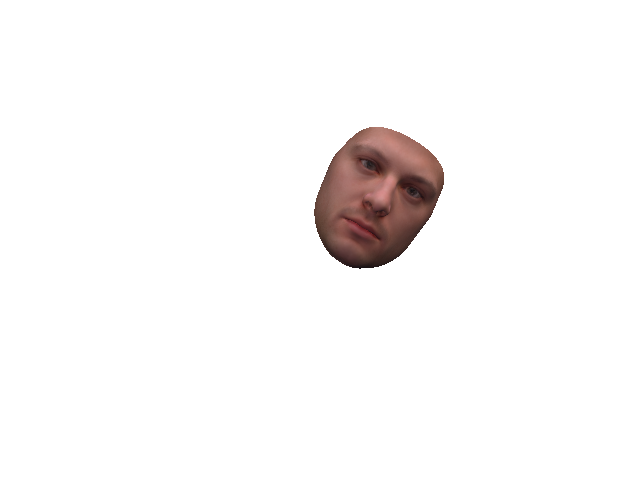
\includegraphics[width=0.99\textwidth]{Figures/dataset/2D/7.png}
    \end{minipage}
    \caption{A visual comparison of our method and the standard 2D fitting results.}
    \label{f4.5}
\end{figure}

% overly
\begin{figure}[h]
    \centering
    \begin{minipage}{.325\textwidth}
      \centering
      \caption*{Target}
      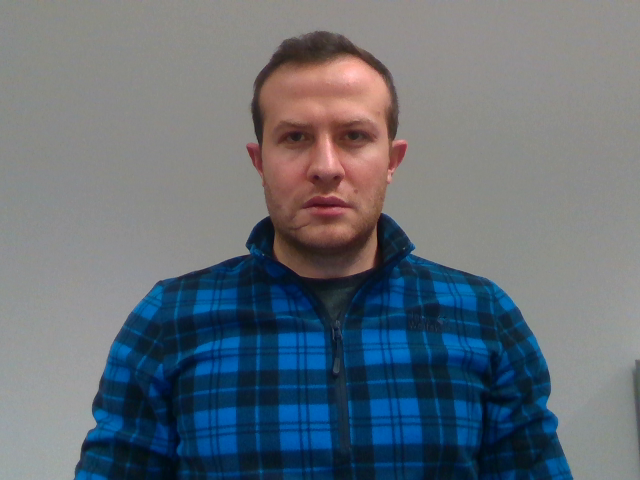
\includegraphics[width=0.99\textwidth]{Figures/dataset/target/1.png}
    \end{minipage}
    \begin{minipage}{.325\textwidth}
      \centering
      \caption*{Our fit overlaid}
      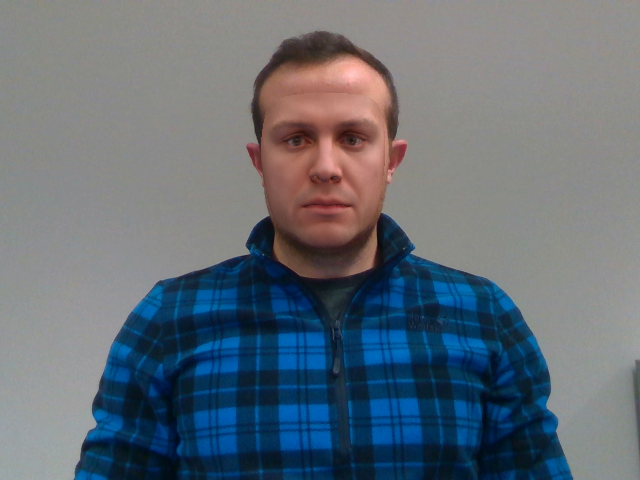
\includegraphics[width=0.99\textwidth]{Figures/dataset/our/1blended.png}
    \end{minipage}
    \begin{minipage}{.325\textwidth}
      \centering
      \caption*{Standard fit overlaid}
      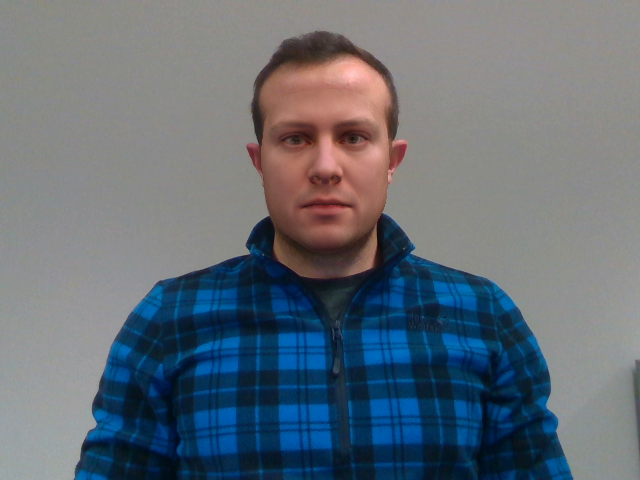
\includegraphics[width=0.99\textwidth]{Figures/dataset/blended/1.png}
    \end{minipage}

    \begin{minipage}{.325\textwidth}
      \centering
      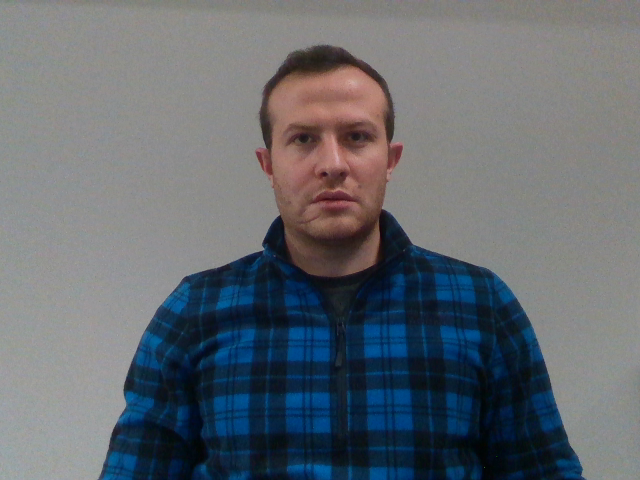
\includegraphics[width=0.99\textwidth]{Figures/dataset/target/3.png}
    \end{minipage}
    \begin{minipage}{.325\textwidth}
      \centering
      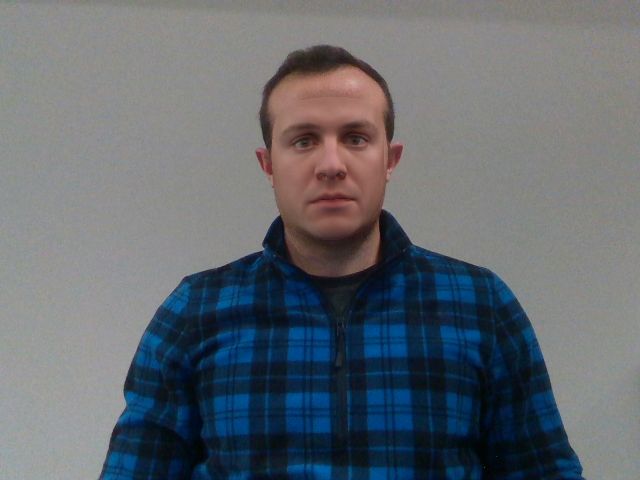
\includegraphics[width=0.99\textwidth]{Figures/dataset/our/3blended.png}
    \end{minipage}
    \begin{minipage}{.325\textwidth}
      \centering
      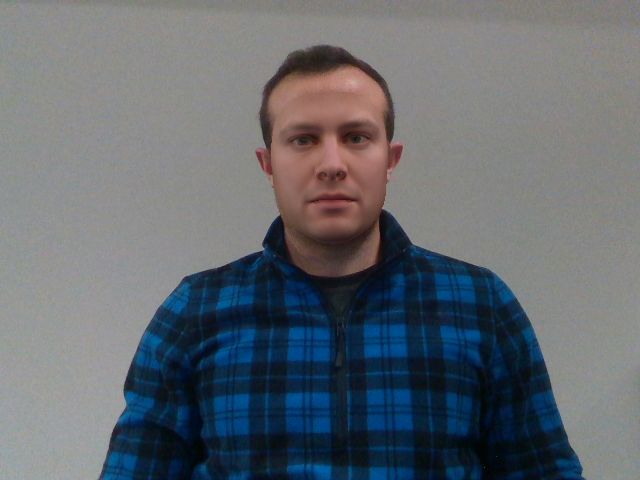
\includegraphics[width=0.99\textwidth]{Figures/dataset/blended/3.png}
    \end{minipage}

    \begin{minipage}{.325\textwidth}
      \centering
      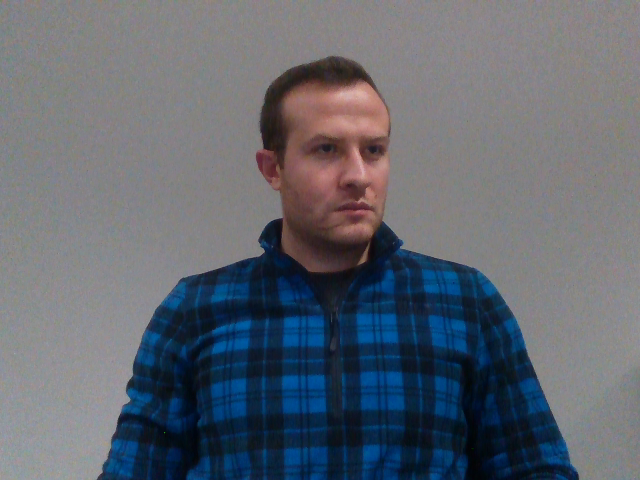
\includegraphics[width=0.99\textwidth]{Figures/dataset/target/4.png}
    \end{minipage}
    \begin{minipage}{.325\textwidth}
      \centering
      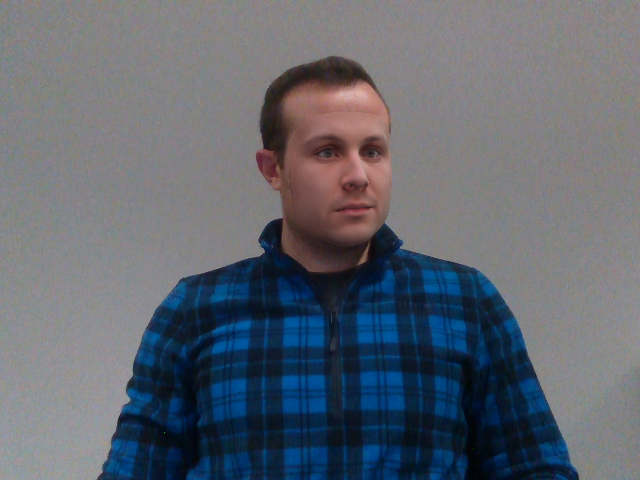
\includegraphics[width=0.99\textwidth]{Figures/dataset/our/4blended.png}
    \end{minipage}
    \begin{minipage}{.325\textwidth}
      \centering
      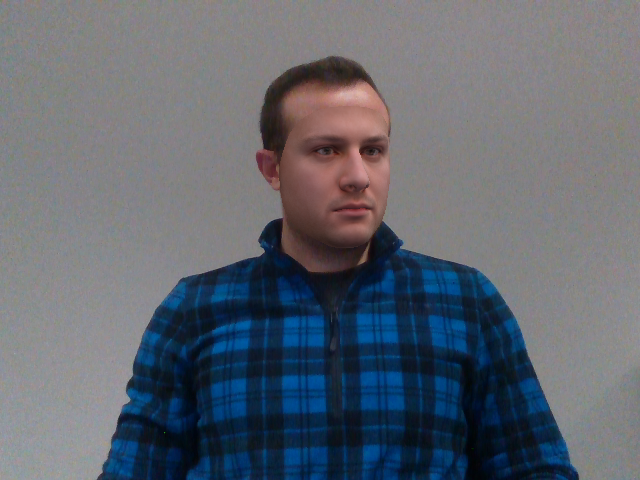
\includegraphics[width=0.99\textwidth]{Figures/dataset/blended/4.png}
    \end{minipage}

    \begin{minipage}{.325\textwidth}
      \centering
      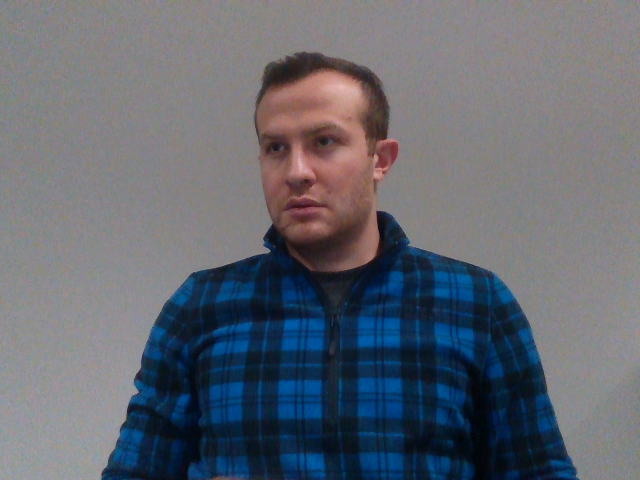
\includegraphics[width=0.99\textwidth]{Figures/dataset/target/5.png}
    \end{minipage}
    \begin{minipage}{.325\textwidth}
      \centering
      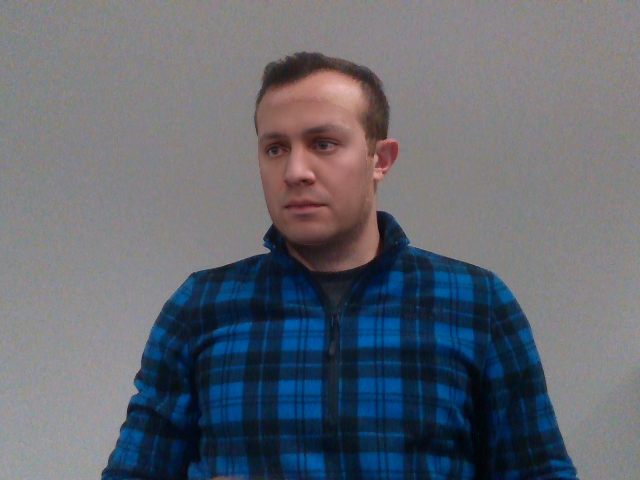
\includegraphics[width=0.99\textwidth]{Figures/dataset/our/5overlay.png}
    \end{minipage}
    \begin{minipage}{.325\textwidth}
      \centering
      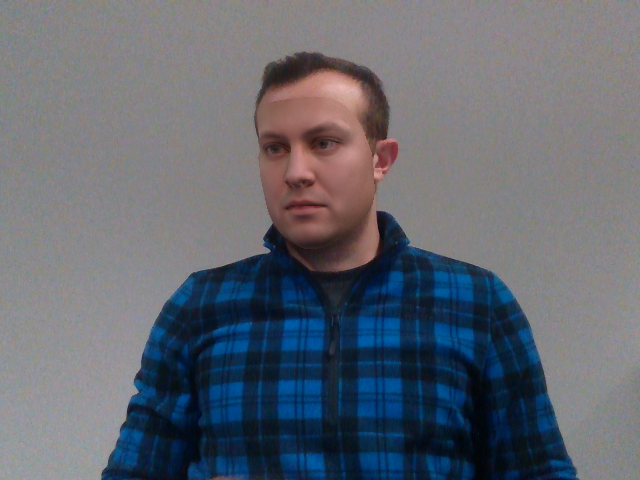
\includegraphics[width=0.99\textwidth]{Figures/dataset/blended/5.png}
    \end{minipage}

    \begin{minipage}{.325\textwidth}
      \centering
      \includegraphics[width=0.99\textwidth]{Figures/dataset/target/6.png}
    \end{minipage}
    \begin{minipage}{.325\textwidth}
      \centering
      \includegraphics[width=0.99\textwidth]{Figures/dataset/our/6blended.png}
    \end{minipage}
    \begin{minipage}{.325\textwidth}
      \centering
      \includegraphics[width=0.99\textwidth]{Figures/dataset/blended/6.png}
    \end{minipage}

    \begin{minipage}{.325\textwidth}
      \centering
      \includegraphics[width=0.99\textwidth]{Figures/dataset/target/7.png}
    \end{minipage}
    \begin{minipage}{.325\textwidth}
      \centering
      \includegraphics[width=0.99\textwidth]{Figures/dataset/our/7blended.png}
    \end{minipage}
    \begin{minipage}{.325\textwidth}
      \centering
      \includegraphics[width=0.99\textwidth]{Figures/dataset/blended/7.png}
    \end{minipage}
    \caption{A  visual comparison of the same fits from Figure \ref{f4.5} overlaid to the target image.}
    \label{f4.6}
\end{figure}
\clearpage
\begin{figure}
  \centering
  \includegraphics[width=0.99\textwidth]{Figures/standard.pdf}
  \caption{The average mesh distance comparison of our method(1st and 2nd column) and the standard fitting method(3rd and 4th column).}
  \label{f4.4}
\end{figure}

\section{Execution Performance}
In order for our system to be useful for demo applications the execution time of at least one module needs to be reduced down to seconds. While it was not possible for us to achieve a decent full fitting performance time-wise. We were able to execute shape fitting module within the reasonable time limits (bellow 30 seconds). We show average execution times for each module in Table \ref{t4.4}. 

\begin{table}[h]
  \centering
  \begin{tabular}{ c|c|c }
      Module  & \#Iterations & Avg. Execution time \\
      \hline
      Shape Fitting   & 500  & $\thicksim$ 25 seconds\\
      Shape Fitting   & 1000 & $\thicksim$ 45 seconds\\\hline
      Full Fitting (Shape + Color Fitting)   & 5000 & $\thicksim$ 10 minute \\
      Full Fitting (shape + Color Fitting)   & 10000 & $\thicksim$ 18 minute \\
      \hline
  \end{tabular}
  \caption{Timing the execution times for shape fitting and color fitting module.}
  \label{t4.4}
\end{table}

\section*{Web-Service Integration}

Based on shown results, the shape fitting does have the potential of being used for demonstration purposes and it is possible to integrate into the Scalismo Face Morpher web-service. Obviously, listed times are directly dependent on sampling iterations, increasing them will increase the execution time and decreasing will reduce time alongside with quality of the reconstruction. To be able to integrate our proposed shape fitting procedure into the current web client we have implemented a single intermediate Thrift server which will connect the already existing Face Morpher web module and proposed shape fitting module to each other. The flow of this system can be seen in Figure \ref{f4.7}.

\begin{figure}
  \centering
  \includegraphics[width=\textwidth]{Figures/web-fitting.pdf}
  \caption{Connecting web client to our proposed fitting modules using the single intermediate server. Everything that is inside the orange box is part of our fitting pipeline.}
  \label{f4.7}
\end{figure}

Whenever a user triggers the starting sequence, the web client sends the request to the intermediate server. The server, that has our fitting pipeline embedded into it as a library, then calls a method from our pipeline which triggers the fitting client to send a request to the camera module in order to obtain the data and start the shape fitting procedure. Due to these multiple client-server interactions, the overall execution time will increase slightly but it will still stay in an acceptable region. 